\section{Konjunkturpolitik}
\subsection{Klassiker}
Zentrale Aussage: Das Angebot ($A$) bestimmt die Konjunktur:
\begin{equation*}
		\mbox{BIP} = f(A)
\end{equation*}
 

\begin{itemize}\itemsep0em
	\item gehen auf Adam Smith zurück
	\item glauben, der Markt regle sich aufgrund des Preis-Zinsmechanismusses selbst (\enquote{unsichtbare Hand})
	\item wollen deshalb, dass sich der Staat hat die Rolle \enquote{Nachtwächters} beschränkt 
	\item halten das Angebot für vollkommen unelastisch (senkrecht) d.\,h. Preisänderungen haben keinen Einfluss auf das Angebot
	\item glauben, Arbeitslosigkeit sei stets freiwillig
\end{itemize}

\subsection{Keynesianismus}\itemsep0em
Zentrale Aussage:  Die Nachfrage ($N$) bestimmt die Konjunktur: 
\begin{equation*}
	\mbox{BIP} =f(N)
\end{equation*}
\begin{itemize}\itemsep0em
	\item geht auf John Mac Keynes (\enquote{längerfristig sind wir alle tod}) zurück 
	\item entstand aus der Massenarbeitslosigkeit in der 1930er Jahren (Nachfrage $<$ Angebot $\Rightarrow$ Nachfragelücke $\Rightarrow$ weniger Produktion $\Rightarrow$ noch mehr Arbeitslose)
	\item sieht den Markt sei nicht im Gleichgewicht, weil es sich beim Geldkreislauf um ein offenes System handelt:
	\begin{center}
		\begin{tikzpicture}[node distance=0.35cm, auto]
		%nodes
		\node[punkt] (haushalt) {Haushalte};
		\node[above left=of haushalt] (import) {Importe};
		\node[left=of haushalt] (sparen) {Sparen};
		\node[below left=of haushalt] (steuern) {Steuern};
		\node[punkt, inner sep=5pt,right=0.45cm of haushalt] (unternehmen) {Unternehmen};
		\node[above right=of unternehmen] (exporte) {Exporte};
		\node[right=of unternehmen] (investition) {Investitionen};
		\node[below right=of unternehmen] (staat) {Subventionen};
		\path 
			(unternehmen.south) edge[pil,bend left=45] node[below]{Löhne} (haushalt.south) 
			(haushalt.north) edge[pil, bend left=45] node[above]{Einkäufe} (unternehmen.north) 
			(haushalt) edge[pil] (import)
			(haushalt) edge[pil] (steuern)
			(haushalt) edge[pil] (sparen)
			(exporte) edge[pil] (unternehmen)
			(investition) edge[pil] (unternehmen)
			(staat) edge[pil] (unternehmen);
		\end{tikzpicture}
	\end{center}
	\item hält Preise für starr, weil Preisänderungen mit Kosten verbunden sind (menu-costs). Somit ist das Angebot flach (waagrecht)
	\item versucht die Liquiditäs- und Investitionsfalle zu umgehen
	\item will, dass der Staat in Krisenzeiten die Nachfrage belebt (z.\,B. durch Bau eines neuen Gotthardtunnels) was folgende Probleme mit sich bringt:
	\begin{itemize}\itemsep0em
		\item Timelag: Staatliche Entscheidungen werden verzögert getroffen
		\item Kurzfristigkeit: staatliche Investionen wirken nur kurzfristig
		\item Rückweg: In der Hochkonjunktur müssten die Steuern erhöht werden (werden sie aber i.\,d.\,R. nicht)
		\item Crowding out: private Investitionen werden durch staatliche verdrängt
	\end{itemize}
	\item empfehlen für den Staat ein antizyklisches Verhalten
\end{itemize}


\subsection{Monetarismus}\itemsep0em
Zentrale Aussage: Die Geldmenge/-poltitk steuert die Konjunktur
\begin{itemize}\itemsep0em
	\item geht auf Milton Friedman zurück
	\item entstand als Reaktion auf die Hyperinflation nach WW2
	\item zielt darauf ab, Inflation um jeden Preis zu vermeiden
	\item will, dass sich Geld- und Gütermenge gleich entwickeln (Quantitätsgleichung)
	\item will keine antizyklische Finanzpolitik
	\item will einen konjunkturneutralen Finanzhaushalt 
	\item ist die herrschende Lehre in Deutschland
	\item hat Einfluss auf die Schweiz
\end{itemize}


\subsection{Angebotsökonomen}
Zentrale Aussage: Weniger Staat, mehr Markt
\begin{equation*}
	\mbox{BIP} =  f(A)
\end{equation*}

\begin{itemize}\itemsep0em
	\item gehen auf Arthur Laffer zurück
	\item entstanden durch die Ölkrise der 1970er Jahre
	\item wollen möglichst gute Bedingungen für Unternehmen
	\item wollen nicht Krisen bekämpfen, sondern für langfristiges Wachstum sorgen
	\item behaupten (Laffer-Kurve), das geringere Steuersätze zu mehr Steuereinnahmen führen
	\begin{center}
	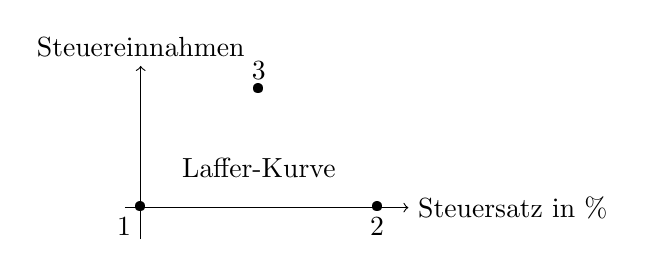
\begin{tikzpicture}[yscale=2, domain=0:3]
		%\draw[very thin,color=gray] (-0.1,-1.1) grid (8.9,1.9);
		\draw[->] (-0.2,0) -- (3.4,0) node[right] {Steuersatz in \%};
		\draw[->] (0,-0.2) -- (0,0.9) node[above] {Steuereinnahmen};
		\draw[thick, domain=0:3]  plot [id=x] function {-x*x/3+x};
		\draw (0, 0) node {\textbullet} node [below left] {1};
		\draw (3, 0) node {\textbullet} node [below] {2};
		\draw (1.5, 0.75) node {\textbullet} node [above] {3};
		\draw (1.5, 0.25) node {Laffer-Kurve};
	\end{tikzpicture}
	\end{center}
	\begin{itemize}\itemsep0em
		\item [1] Keine Steuern, keine Einnahmen
		\item [2] 100\% Steuern, auch keine Einnahmen, weil niemand arbeitet
		\item [3] Maximale Steuereinnahmen
	\end{itemize}
	\item haben Einfluss in Deutschland und in der Schweiz
\end{itemize}

\subsection{Neoklassiker}
Zentrale Aussage: Staatliche Eingriffe sind der Anfang allen Übels
\begin{itemize}\itemsep0em
	\item gehen auf Friedrich August von Hayek zurück
	\item wollen, dass nicht auf Kredit investiert wird
	\item gehen vom Homo oeconomicus aus	
	\item glauben an die \enquote{unsichtbare Hand}
	\item glauben an den vollkommenen Markt
\end{itemize}

\subsection{Tatsächliches Verhalten der Preise}
Langfristig sind Preise flexibel, kurzfristig sind sie starr.

\subsection{Rettung Griechenlands}
Steuern senken, staatliche Investitionen senken, Zinsen senken.
Wird aber nicht gemacht -- die Griechen sollen erst richtig leiden, dann ihre Mentalität ändern.